
\documentclass[sigconf]{acmart}
\usepackage{graphicx}
\usepackage{enumerate}

%%
%% \BibTeX command to typeset BibTeX logo in the docs
\AtBeginDocument{%
	\providecommand\BibTeX{{%
			\normalfont B\kern-0.5em{\scshape i\kern-0.25em b}\kern-0.8em\TeX}}}

%% Rights management information.  This information is sent to you
%% when you complete the rights form.  These commands have SAMPLE
%% values in them; it is your responsibility as an author to replace
%% the commands and values with those provided to you when you
%% complete the rights form.
\setcopyright{acmcopyright}
\copyrightyear{2018}
\acmYear{2018}
\acmDOI{10.1145/1122445.1122456}

%% These commands are for a PROCEEDINGS abstract or paper.
\acmConference[Woodstock '18]{Woodstock '18: ACM Symposium on Neural
	Gaze Detection}{June 03--05, 2018}{Woodstock, NY}
\acmBooktitle{Woodstock '18: ACM Symposium on Neural Gaze Detection,
	June 03--05, 2018, Woodstock, NY}
\acmPrice{15.00}
\acmISBN{978-1-4503-XXXX-X/18/06}


\begin{document}
	
	\title{Improving open domain question answering with Knowledge Base and Wikipedia graph}
	
	
	
	
	\begin{abstract}
		A clear and well-documented \LaTeX\ document is presented as an
		
	\end{abstract}
	
	\keywords{ neural networks}
	
	\maketitle
	
	\section{Introduction}
	Open-domain  Question Answering mostly focus on factoid question answering,which require systems to return a short and concise answer to these questions.
	Most existing models, however,answer questions using a single information
	source, usually either text from an text corpus such as Wikipedia\cite{chen2017reading},or a single knowledge base (KB).	
	
	Large-scale factual knowledge bases such as WikiData\cite{vrandevcic2014wikidata},Freebase \cite{bollacker2008freebase},Dbpedia\cite{auer2007dbpedia}, stores a large number of facts in an organized way. Namely, Freebase has 46m entities and 2.6b facts, WikiData contains 87m items .Each fact is made of two entities and a relation between them. Most konwledge bases are curated,ensureing the correctness of the information,common or "simple" questions can be answered easily if semantic parsing (question query)  is done correctly.The advantage of graph structure also enables multi-hop question answering.
	Unfortunately, curated konwledge bases, which demands tremendous hunman labor,might not keep up with times,\\thereby some relations would be missing.Limited coverage of questions  can be answered because the resoning is based on the similarity over relationships and entities.	
	
	Wikipedia\cite{chen2017reading}, a text source, was proposed for the first time to process Open Domain QA tasks, and a DRQA system was developed, including Document Retriever and Document Reader, which laid the pipe-line, two-stage approaches, of QA for successive work.\\We also follow this tradition ,retrieve and then read. 		
	Text corpus provides a more completed coverage of facts,and it is easier to catch the time, however lacks the ability of multi-hop resoning.
	
	To combine the coverage of text evidence and reasoning ability of knowledge base, some recent work  use both text and KB,to constructs graphs of nodes and edges\cite{sun2018open,sun2019pullnet,xiong2019improving}.These works basically augment the KB graph with the entities indentified from the relevent text evidences,the task of answer determination is then reduced to classfiy the entity node is the answer or not.
	Another line\cite{min2019knowledge,ding2019cognitive} ,inversely,augment retrieval passage with KB graph, and the task of answer determination is to do answer extraction from text.
	
	\section{Related work}
	\subsection{QA using Text}
	Cognitive Graph\cite{ding2019cognitive}retrieves evidence documents offline, and trains a reading comprehension model to jointly predict possible answer spans and next-hop spans to extend the reasoning chain. \cite{asai2019learning}learns to sequentially retrieve evidence paragraphs over the Wikipedia graph  by conditioning on the previously retrieved documents.They constructs Wikipedia graph offline and  reused it throughout training and inference for any question.We will use this new meta resource in our work.
	\subsection{QA using KB}
	\subsection{QA using both Text and KB}
	In \cite{sun2018open,sun2019pullnet,xiong2019improving},the  answers is restricted to be the KB entities. GRAFT-Net \cite{sun2018open} constructs a heterogeneous question subgraph, which contains  KB triples(entity,relation,entity), and entity-linked text. Afterwards, PullNet \cite{sun2019pullnet} expands more  entities from relevant documents to form a isomorphic graph. The task of QA then reduces to learning the representations of the nodes, and then performing a binary classification over these nodes to decide whether it is the answer or not. They both augmented knowledge bases with text from Wikipedia,the text here plays an auxiliary role.
	
	However,\cite{min2019knowledge} construct the graph in a different way.  Inversely, the knowledge base is used to better model relationships between different passages of text. It use KB relations to formulate entity-introductory-passage relations. The task of QA  switches to learning the KB-aware representations of  passages . Not to classify the node is the answer or not, it extracts the most possible span as answer in the most possible passage as prior work did.Our work is consistent with it but with different approach.
	
	\section{Method}
	Specifically, we use Wikipedia graph\cite{asai2019learning}
	as the text corpus $\mathcal{G}$ and Wikidata\cite{vrandevcic2014wikidata}  as the knowledge base $\mathcal{K}$, as there exists an alignment between the two resources.
	Knowledge Base is a multi-relational graphs, each edge has a label and direction associated with it, and each node in the graph is an entity.
	Wikipedia graph\cite{asai2019learning} is a directed graph,constructed by hyperlinks and within-document links, each node represents a single paragraph.The Wikipedia graph is densely connected and covers a wide range of topics that provide useful evidence for open-domain questions.
	Our goal is to fuse Knowledge Base knowledge into Wikipedia graph passages,learn the KB-aware representation of all the retrieved passage, as the input to a reader model to extract answer.
	
	\textbf{Seed Nodes}  Given a natural language question $q$,we use the top $K_{TF-IDF}$ paragraphs  returned by a TF-IDF based retrieval system as the start nodes. 
	
	\textbf{Subgraph}
	Next,we run Topic-sensitive pagerank\cite{haveliwala2003topic} around these seed nodes  to get the edges weight over their neighbouring, denoted as  $\mathcal{G}_q = (\mathcal{P},\mathcal{E})$,where $\mathcal{P}$ is the set of paragraphs $\left\{p_1,...,p_{|p|}\right\}$ in the Wikipedia graph, and the edge $\mathcal{E}$ are links between them with a pagerank score $pr$ over them.Each paragraphs is a
	sequence of words $p_i = (w_1^{p_i},...,w_{|pi|}^{p_i})$
	
	\textbf{Node Initialization}
	Note that 	we use the same encoder BERT during the whole process.
	\begin{enumerate}[(1)]
		\item Question initialization\\
		Given a natural language question $q = (w_1^q,...,w_q^q)$,initialize question as:
		\begin{displaymath}
			\begin{aligned}
				h_q^{(0)} = BERT(w_1^q,...,w_{|q|}^q)				
			\end{aligned}
		\end{displaymath}
		We perform an entity linking system\cite{ferragina2011fast} to identity the \emph{topic entity} in the question,denoted as $E_{topic}=\left\{e_1,...,e_{|topic|}\right\}$.
		
		\item Passage initialization\\
		And the passages in $\mathcal{G}_q$ are initialized as:
		\begin{displaymath}
			\begin{aligned}
				h_{p_i}^{(0)} = BERT(w_1^{p_i},...,w_{|pi|}^{p_i})				
			\end{aligned}
		\end{displaymath}	
		We denote  the embedding of  \emph{pos-th} word in the passage $p_{i}$ as $h^{(l)}_{pi}[pos]$.
		
	\end{enumerate}
	
	\textbf{Node Update}		
	Assuming that $(p_a,p_b) \in \mathcal{G}_q$, and the edge weight is $pr_{a,b}$, we also perform an entity linking system\cite{ferragina2011fast} to identity the  entity in $p_a$ and $p_b$.Suppose that		
	$p_a$ contains n entities ( $e_{a1},...,e_{an}$) ,		
	$p_b$ contains m entities ( $e_{b1},...,e_{bm}$) .In each layer $l$,we update the information as follow:
	\begin{enumerate}[(1)]
		\item Corperate entity relations into passage .\\	
		We update passage representaion at token level.	
		If the triple $(e_{ai},r,e_{bj}) \in \mathcal{K}$, and $e_{ai}$ is at the position $pos_a$ in $p_a$, $e_{bj}$ is at  $pos_b$  in $p_b$,		
		let $L=(p_a,pos_a)$ be the set of all the entities appearing at position $pos_a$ in paragrah $p_a$,they are all linked to the entities at position $pos_b$ in paragrah $p_b$.We aggregate over the token hidden states coming in at
		each position separately: 
		
		\begin{displaymath}
			\begin{aligned}
				h^{(l)}_{p_b}[pos_b] = FFN
				\left(					 
				\begin{bmatrix}  
					h^{(l-1)}_{p_b}[pos_b],\\ 		
					\sum\limits_{(p_a,pos_a) \in L}
					pr_{a,b}*
					s(h_r,h_q^{(l)})*
					\phi(h^{(l-1)}_{p_a}[pos_a],h_r)
				\end{bmatrix} 
				\right)								
			\end{aligned}
		\end{displaymath}
		
		$s(h_r,h_q^{(l)})$ is the relevant score between relation and question,we simply computes it through the dot product between their hidden state.$h_r$ is embedding of  relations,which are pretrained and can be looked up from an embedding table.
		\begin{displaymath}
			\begin{aligned}
				s(h_r,h_q^{(l)}) = h_r\dot{h_q^{(l)}}
			\end{aligned}
		\end{displaymath}
		$\phi$ is a transform operation,which is 
		\begin{displaymath}
			\phi(h,r) = FFN(h;r)
		\end{displaymath}
		
		\item Update passage representation\\
		Next we aggregate states within the paragraph using BERT again:
		\begin{displaymath}
			\begin{aligned}
				h_{p}^{(l)} = BERT(h_p^{(l)}[1],...,h_p^{(l)}[|p|])
			\end{aligned}
		\end{displaymath}
		
		\item Update topic entities representation\\
		We have $E_{topic}=\left\{e_1,...,e_{|topic|}\right\}$ from above step. 
		Let $Q = \left(e,p,pos\right)$ denotes the topic entity $e$ appear at the position $pos$ in passage p,we update the topic entity representation by aggregate the information from the updated passages.
		\begin{displaymath}
			\begin{aligned}
				h^{(l)}_{e} = \frac{1}{|Q|}\sum\limits_{(e,p,pos) \in Q} h_p^{(l)}[pos]
			\end{aligned}
		\end{displaymath}
		
		\item Update question representation\\
		Next we aggregate states within the qusetion using BERT again:
		\begin{displaymath}
			\begin{aligned}
				&h_{q}^{(l)} = BERT(h_q^{(l)}[1],...,h_q^{(l)}[pos])\\
				&s.t.\\
				&h_q^{(l)}[i] = \left\{
				\begin{aligned}
					&h^{(l)}_{e}  		 , & {\Phi(e,i) = 1} \\
					&h_q^{(l-1)}[i]     ,& { \Phi(e,i) = 0 }
				\end{aligned}
				\right.
			\end{aligned}
		\end{displaymath}
		$\Phi(e,i)=1$ means the token at position i in question  is a topic entity.
		
		
		
		\textbf{ Answer Extraction }\\		
		Denote the passage score as $Pr(P_i|Q, P)$,which reranks all retrieved passages
		\begin{displaymath}
			Pr(P_i|Q, P) = softmax( W[h_{pi}^\mathrm{ T };h_q] )
		\end{displaymath}
		
		$W$ is a trainable parameter.
		
		The score of an answer span from passage $\MakeUppercase{p}_i$ will be
		\begin{displaymath}
			Pr(a| Q, P) = 	Pr(P_i|Q, P)P_s(a_s|Q, P)P_e(a_e|Q, P).
		\end{displaymath}
		
	\end{enumerate} 
	\begin{figure*}[ht]		
		\centering
		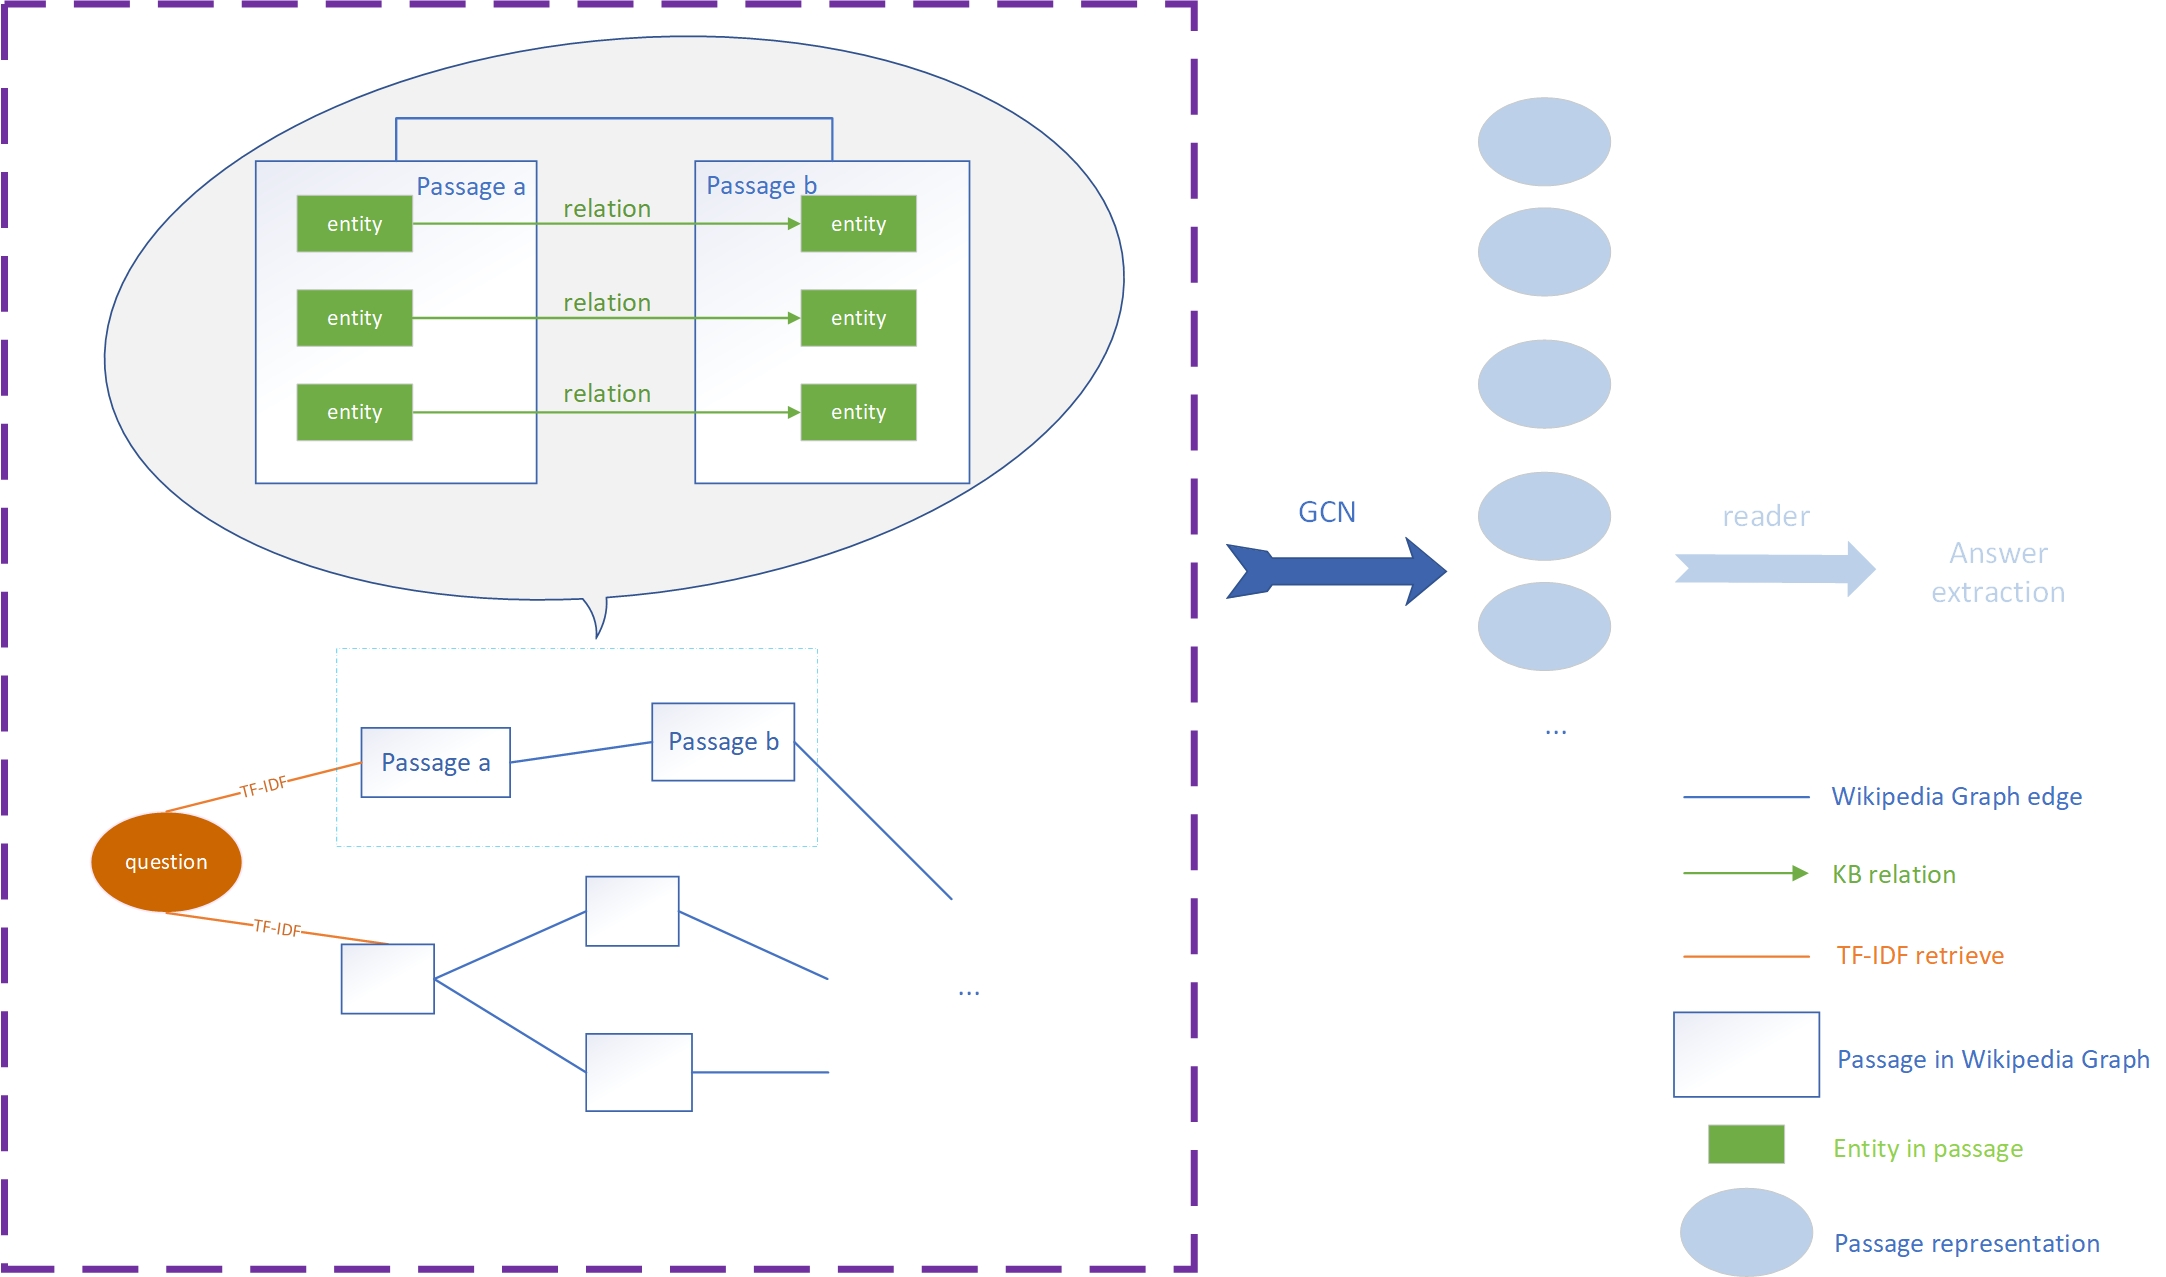
\includegraphics[scale=0.6]{f1.jpg}
		\caption{A diagram of approach}
		\label{fig:label}
	\end{figure*}
	
	
	
	
	%%
	%% The next two lines define the bibliography style to be used, and
	%% the bibliography file.
	\bibliographystyle{ACM-Reference-Format}
	\bibliography{refs}
	
	
	
\end{document}
\endinput
%%
%% End of file `sample-sigconf.tex'.
